\documentclass[a4paper]{article}

\usepackage[utf8]{inputenc}
\usepackage[T1]{fontenc}
\usepackage{textcomp}
\usepackage[dutch]{babel}
\usepackage{amsmath, amssymb}
\usepackage{code}
\usepackage{pythonhighlight}

% figure support
\usepackage{import}
\usepackage{xifthen}
\pdfminorversion=7
\usepackage{pdfpages}
\usepackage{transparent}
\usepackage{graphicx}
\usepackage{hyperref}
\pdfsuppresswarningpagegroup=1
\graphicspath{{./img/}}

\begin{document}
\section{trial and tribulations of rolling out a robotic fleet}
\begin{itemize}
	\item Hardware expensive and time taking
	\item work with manufacturer
	\item outdoor robotics is difficult
	\item Dont reinvent wheel (Plan for wxisting solution)
	\item Focus on goal
	\item waterproofing sensor
	\item heat genereate moisture in camera
	\item field testing (moving out things and lockdown)
	\item remote testing (much more effictive)
	\item always have a plan in field testing
	\item pre prep the hardwares(baterry compiled code )
	\item Record every thing
	\item \textbf{Plotjuggler} - important tool for graph visulasation
	\item make nodes anonymous (Shutdown nodes is a pain)
\end{itemize}
\subsection{Principles}
\begin{itemize}
	\item Use standard ros messages
    \item use params and cfg liberally (mainly for cpp codes) 
    \item make simulation more real(messages and other stuff not gfx)
    \item use standard tools 
\end{itemize}
\begin{figure}[htpb]
	\centering
	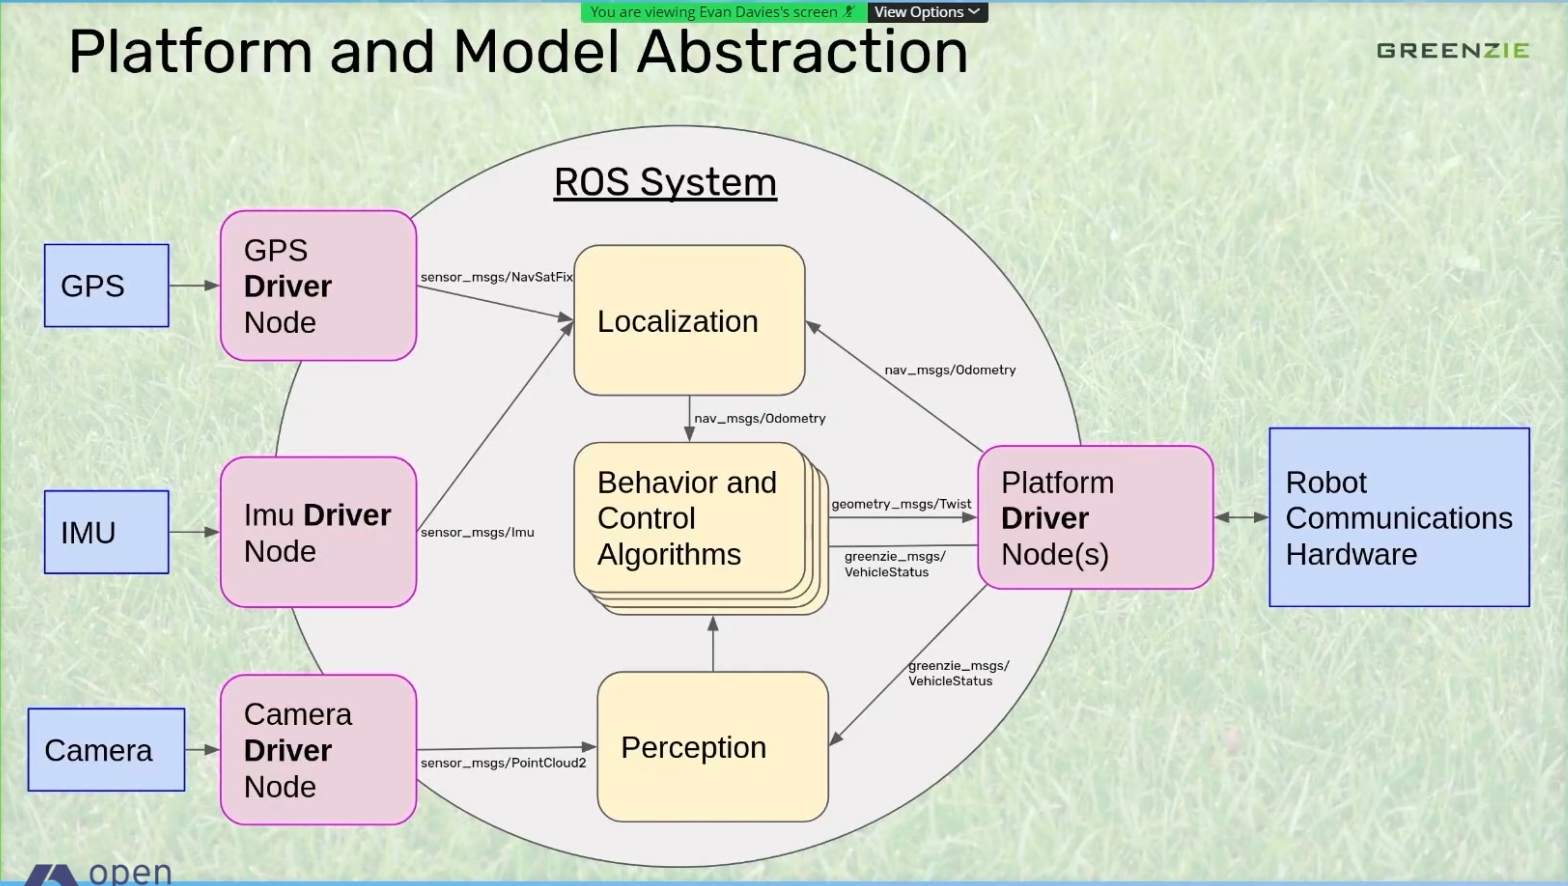
\includegraphics[width=0.5\textwidth]{platform_abstraction.png}
	\caption{}
	\label{fig:}
\end{figure}
\subsection{conclusion}
\begin{itemize}
    \item hardware is hard 
    \item remote testing is valuable
    \item add protective meassures in everything(what can go wrong can go wrong)
    \item abstarct as much as hardware as possible
    \item test as many times as possible 1 2
\end{itemize}
\section{RMF based multi robot traffic management}
\textbf{Robot middleware framework}
\begin{itemize}
        \item To navigate to floors and other rooms - need of communication between doors and elevators
        \item \textbf{free\_fleet} - freefleet client is opensource robot fleet management system \url{https://github.com/open-rmf/rmf_demos}
        \item \textbf{Google or-tool}- tool for solving graphs \url{https://developers.google.com/optimization/routing}
        \item creates a detour path when deadlock arises
        \item clobot - korea based startup working multi robot system \url{https://github.com/CLOBOT-Co-Ltd/clober}
\end{itemize}
\end{document}
